\documentclass[a4paper,11pt,twoside,openright]{report}

\usepackage{tikz}
% \definecolor{se_dark_blue}{RGB}{0,103,166} % powerpoint
\definecolor{se_dark_blue}{RGB}{0,96,178} % website
% \definecolor{se_light_blue}{RGB}{119,158,201} % powerpoint
\definecolor{se_light_blue}{RGB}{129,160,225} % website

\usepackage{pdfpages}
\usepackage[utf8x]{inputenc}
\usepackage[strict]{changepage}

\pdfoptionpdfminorversion=6

%% setup listings
\usepackage{listings}
\lstset{
    numbers=left,
    numberstyle=\tiny,
    numbersep=5pt,
    xleftmargin=11pt,
    xrightmargin=4pt,
    frame=single,
    aboveskip=0pt,
    belowskip=-6pt,
    sensitive=true,
    float=!t,
    breaklines=false,
    captionpos=b,
    tabsize=2,
    showstringspaces=false,
    basicstyle=\small\ttfamily,
    morecomment=[l]{//},
    morecomment=[s][\itshape]{/**}{*/}
}

\setlength{\voffset}{-1in}
\setlength{\hoffset}{-1in}

\setlength{\topmargin}{2.5cm}		   
\setlength{\headheight}{0cm}		   
\setlength{\headsep}{0cm}		   
\setlength{\oddsidemargin}{3,3cm}  % innen ein wenig mehr Rand für die Klebebindung
\setlength{\evensidemargin}{2,7cm} % dafür außen ein wenig weniger
\setlength{\textwidth}{15cm}		   
\setlength{\textheight}{23,5cm}		   
\setlength{\parindent}{0cm}

\begin{document}

% Einrücken von Absätzen verhindern und 1.5 Zeilen Absatzabstand
\setlength{\parindent}{0pt}
\setlength{\parskip}{1.5ex plus0.5ex minus0.5ex}

\begin{titlepage}
	\begin{center}
		\huge \textbf{\textsf{Geometric Non-Termination Arguments for Integer Programs}} \\
		\vspace{2cm}
		\LARGE\textbf{\textsc{Bachelor-Thesis}}\\
		\vspace{1cm}
		\normalsize
		vorgelegt am: \today \\
		\vspace{2.5cm}
		\large \textbf{at the Lehr- und Forschungsgebiet Informatik 2}\\
		\large \textbf{Rheinisch Westfälische Technische Hochschule Aachen}\\
		\vspace{3cm}
	\end{center}
	\normalsize{
		\begin{tabular}{ll}
			Name: & {Timo Bergerbusch} \\
			Matrikelnummer: & {344408} \\
			Studiengang: & Informatik\\
			Studienjahrgang: & 2017\\
			Erstgutachter: & {Jera Hensel} \\
			Zweitgutachter: & {Prof. Dr. Noll} \\
		\end{tabular}\\
	}
\end{titlepage} % English cover

%\clearpage
\chapter{Acknowledgement}

% Erklaerung
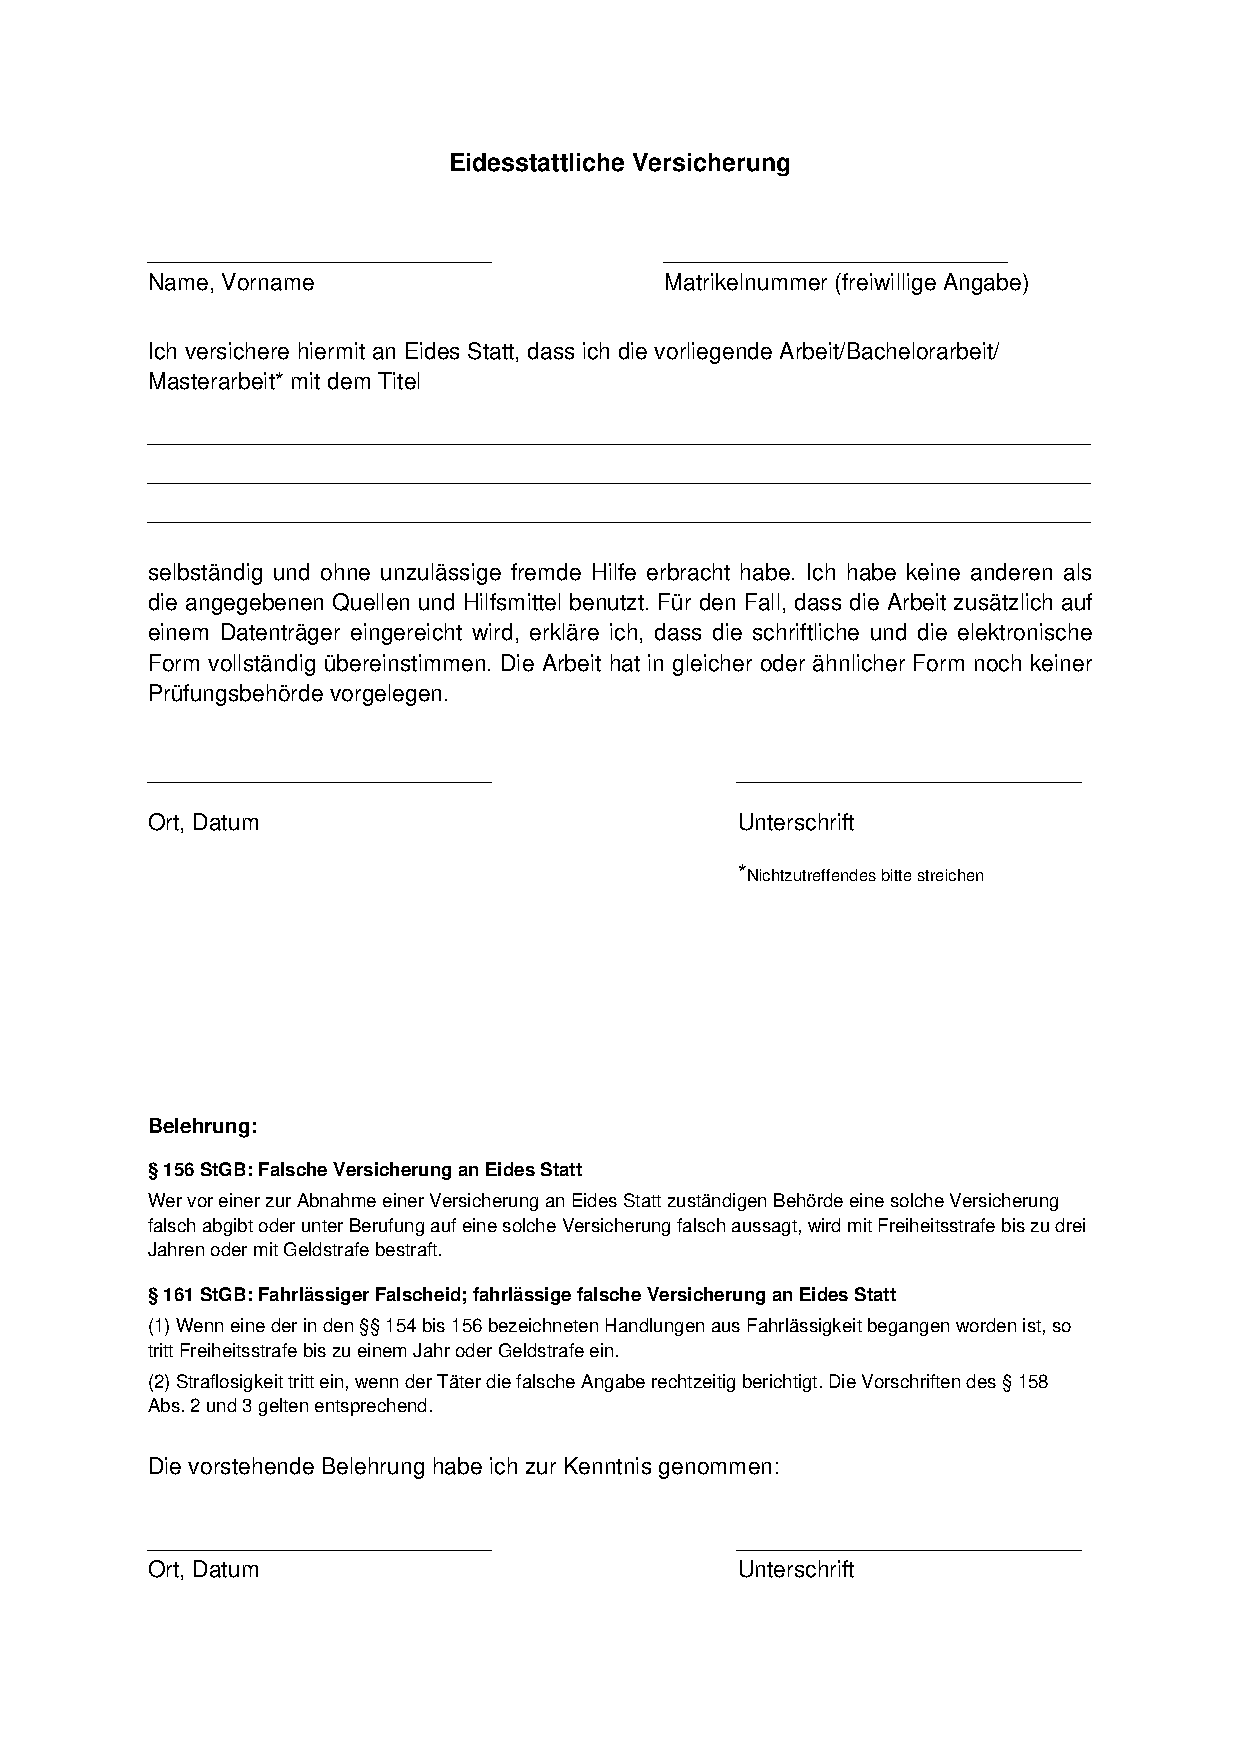
\includepdf[pages={1},offset=-1in -1in]{Formular_Eidesstattliche_Versicherung_neu.pdf}
% \includepdf[pages={1},offset=-1in -1in]{Statutory_Declaration_in_Lieu_of_an_Oath.pdf} % English 

%\clearpage
\chapter{Abstract}

\tableofcontents

% Ab erstem Kapitel Seiten arabisch zählen
\setcounter{page}{1}
\pagenumbering{arabic}

\section{Einleitung}
\frame{\tableofcontents[currentsection]}

\begin{frame} %%Eine Folie
  \frametitle{Einleitung und Motivation}
  \begin{itemize}
  	\item Verbreitung von Software
  	\item Automatische Entwicklungsunterst\"utzung $\Rightarrow$\red{Halte Problem}
  	\item \aprove\newline
	  	\begin{figure}[H]
	  		\centering
		  	\begin{tikzpicture}[scale=0.6, every node/.style={scale=0.6}]
			  	\node[aproveNode] at (0,0) (java) {Java};
			  	\node[aproveNode]at (0,-.75) (c) {C};
			  	\node[aproveNode] at (0,-1.5) (haskell) {Haskell};
			  	\node[aproveNode] at (0,-2.25) (prolog) {Prolog};
			  	\node[shape = circle, draw,align = center] at (3, -1.125) (seg) {Symbolic\\ Execution\\ Graph};
			  	\node<1>[stdNode] at (6,-.75) (its) {\its};			  	
			  	\node<2>[stdNode, color = blue] at (6,-.75) (its) {\its};
			  	\node[stdNode, minimum width = 3cm] at (10,-.25) (comp) {Complexity};
			  	\node[stdNode, minimum width = 3cm] at (10,-1) (term) {Termination};
			  	\node<1>[stdNode, minimum width = 3cm] at (10,-1.75) (nterm) {Non-Termination};
			  	\node<2>[stdNode, minimum width = 3cm, color = blue] at (10,-1.75) (nterm) {Non-Termination};
			  	
			  	\draw[thickarrow] (java) edge (seg);
			  	\draw[thickarrow] (c) edge (seg);
			  	\draw[thickarrow] (haskell) edge (seg);
			  	\draw[thickarrow] (prolog) edge (seg);
			  	
			  	\draw[thickarrow] (seg) edge (its);
			  	\draw[thickarrow] (seg) edge (nterm.west);
			  	
			  	\draw[thickarrow] (its) edge (term);
			  	\draw[thickarrow] (its) edge (comp);
			  	\draw<1>[thickarrow] (its) edge (nterm);
			  	\draw<2>[thickarrow, color = blue] (its) edge (nterm);
			  	
			  	\draw [thick,decoration={brace,mirror},decorate] (-1,-2.75) -- (3.9,-2.75) 
			  	node [pos=0.5,anchor=north,yshift=-0.3cm] {\footnotesize Frontends}; 
			  	
			  	\draw [thick,decoration={brace,mirror},decorate] (5.2,-2.75) -- (11.5,-2.75) 
			  	node [pos=0.5,anchor=north,yshift=-0.3cm] {\footnotesize Backend}; 
		  	\end{tikzpicture}
		\end{figure}
	
  \end{itemize}
\end{frame}

%TODO: mention its derivation
\input{src/tex/Preliminaries}
\chapter{Geometric Non-Termination}

\section{Derivation of the \emph{STEM}}

\section{Derivation of the \emph{LOOP}}

\subsection{The Update Matrix}

\subsection{The Guard Matrix}

\subsection{The Iteration Matrix}

\section{Derivation of the \emph{SMT}-Problem}

\subsection{The Domain Criteria}

\subsection{The Initiation Criteria}

\subsection{The Point Criteria}

\subsection{The Ray Criteria}

\section{Verification of the Geometric Non-Termination Argument}
	 

\chapter{Benchmarks}
\chapter{related work}



\bibliographystyle{alpha}
\addcontentsline{toc}{chapter}{Literaturverzeichnis}
\bibliography{src/bib/Literatur}

% Begin Anhang
\appendix
%\input{src/tex/appendix_docu}

\end{document}
